\documentclass[11pt,a4paper]{report}
\usepackage[textwidth=37em,vmargin=30mm]{geometry}
\usepackage{calc,xunicode,amsmath,amssymb,paralist,enumitem,tabu,booktabs,datetime2,xeCJK,xeCJKfntef,listings}
\usepackage{tocloft,fancyhdr,tcolorbox,xcolor,graphicx,eso-pic,xltxtra,xelatexemoji}

\newcommand{\envyear}[0]{2025}
\newcommand{\envdatestr}[0]{2025-01-04}
\newcommand{\envfinaldir}[0]{webdb/2025/20250104/final}

\usepackage[hidelinks]{hyperref}
\hypersetup{
    colorlinks=false,
    pdfpagemode=FullScreen,
    pdftitle={Web Digest - \envdatestr}
}

\setlength{\cftbeforechapskip}{10pt}
\renewcommand{\cftchapfont}{\rmfamily\bfseries\large\raggedright}
\setlength{\cftbeforesecskip}{2pt}
\renewcommand{\cftsecfont}{\sffamily\small\raggedright}

\setdefaultleftmargin{2em}{2em}{1em}{1em}{1em}{1em}

\usepackage{xeCJK,xeCJKfntef}
\xeCJKsetup{PunctStyle=plain,RubberPunctSkip=false,CJKglue=\strut\hskip 0pt plus 0.1em minus 0.05em,CJKecglue=\strut\hskip 0.22em plus 0.2em}
\XeTeXlinebreaklocale "zh"
\XeTeXlinebreakskip = 0pt


\setmainfont{Brygada 1918}
\setromanfont{Brygada 1918}
\setsansfont{IBM Plex Sans}
\setmonofont{JetBrains Mono NL}
\setCJKmainfont{Noto Serif CJK SC}
\setCJKromanfont{Noto Serif CJK SC}
\setCJKsansfont{Noto Sans CJK SC}
\setCJKmonofont{Noto Sans CJK SC}

\setlength{\parindent}{0pt}
\setlength{\parskip}{8pt}
\linespread{1.15}

\lstset{
	basicstyle=\ttfamily\footnotesize,
	numbersep=5pt,
	backgroundcolor=\color{black!5},
	showspaces=false,
	showstringspaces=false,
	showtabs=false,
	tabsize=2,
	captionpos=b,
	breaklines=true,
	breakatwhitespace=true,
	breakautoindent=true,
	linewidth=\textwidth
}






\newcommand{\coverpic}[2]{
    % argv: itemurl, authorname
    Cover photo by #2~~(\href{#1}{#1})
}
\newcommand{\makeheader}[0]{
    \begin{titlepage}
        % \newgeometry{hmargin=15mm,tmargin=21mm,bmargin=12mm}
        \begin{center}
            
            \rmfamily\scshape
            \fontspec{BaskervilleF}
            \fontspec{Old Standard}
            \fontsize{59pt}{70pt}\selectfont
            WEB\hfill DIGEST
            
            \vfill
            % \vskip 30pt
            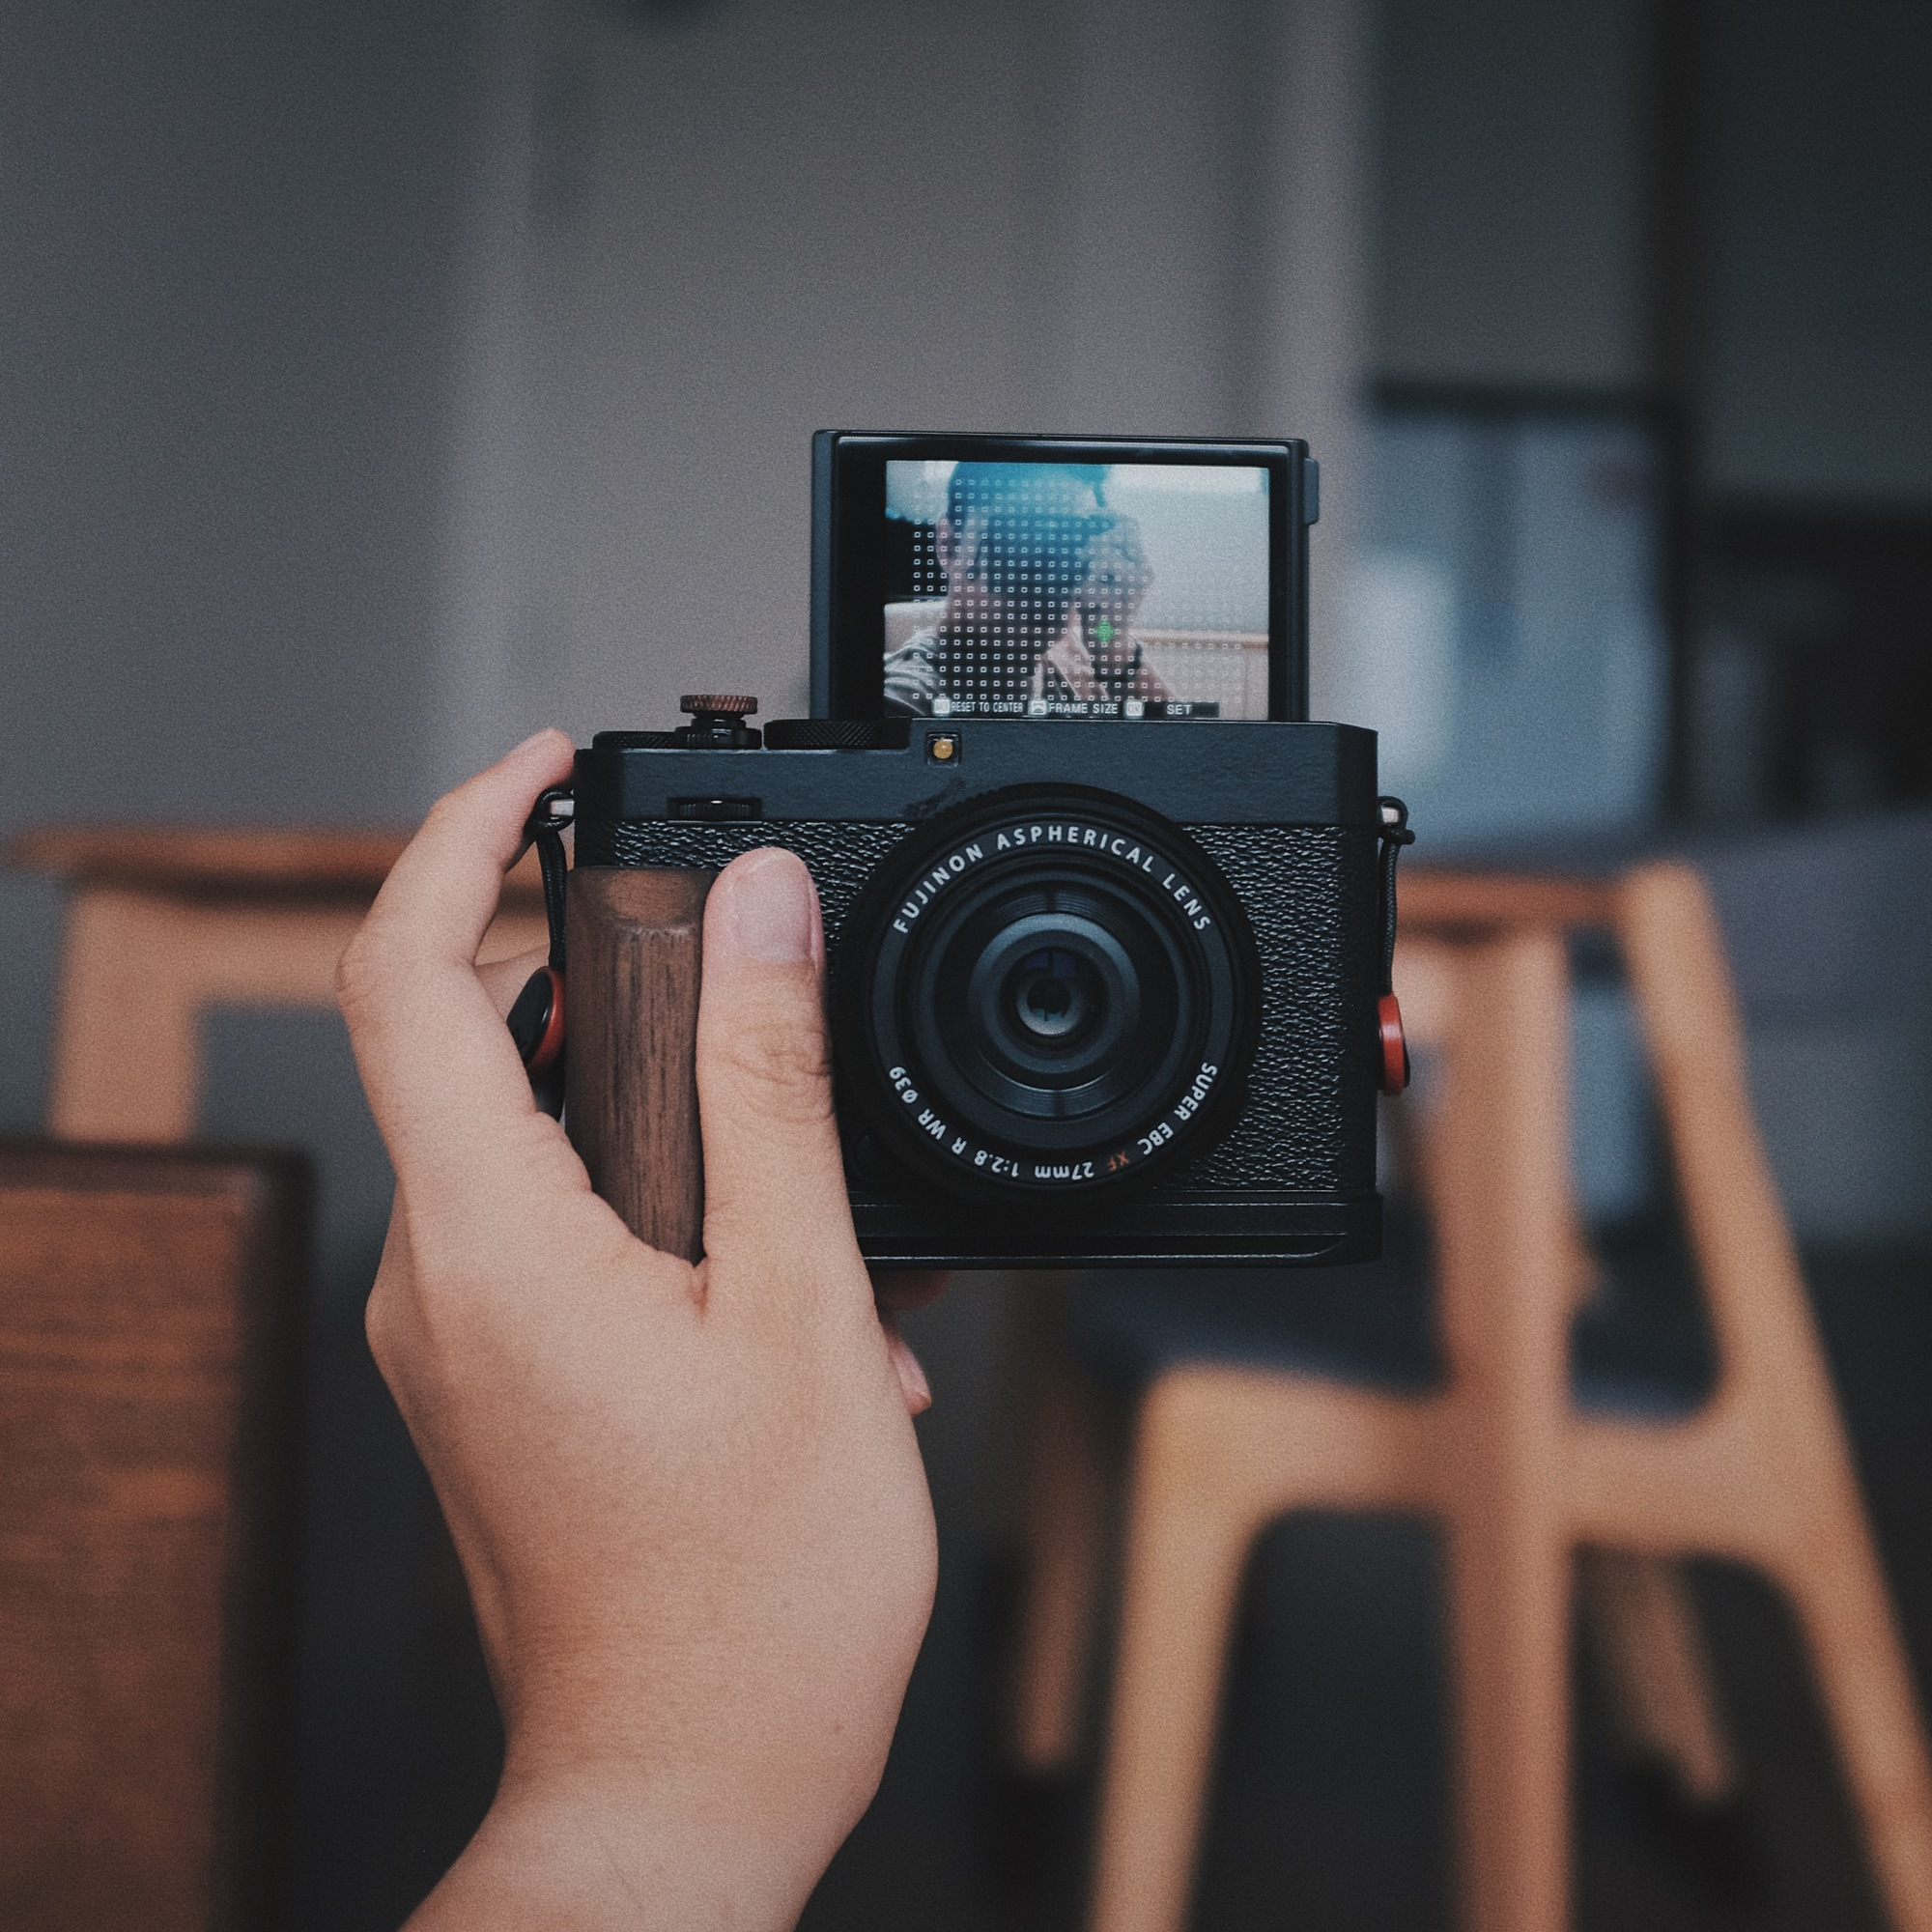
\includegraphics[width=\linewidth]{\envfinaldir/coverpic-prod.jpg}\par
            % \vskip 30pt
            \vfill

            \normalsize\rmfamily\scshape
            \copyright{} The Web Digest Project \hfill\large \envdatestr
        \end{center}
    \end{titlepage}
    % \restoregeometry
}
\newcommand{\simplehref}[1]{%
    \textcolor{blue!80!green}{\href{#1}{#1}}%
}
\renewcommand{\contentsname}{\center\Huge\sffamily\bfseries Contents\par\vskip 20pt}
\newcounter{ipartcounter}
\setcounter{ipartcounter}{0}
\newcommand{\ipart}[1]{
    % \vskip 20pt
    \clearpage
    \stepcounter{ipartcounter}
    \phantomsection
    \addcontentsline{toc}{chapter}{#1}
    % \begin{center}
    %     \Huge
    %     \sffamily\bfseries
    %     #1
    % \end{center}
    % \vskip 20pt plus 7pt
}
\newcounter{ichaptercounter}
\setcounter{ichaptercounter}{0}
\newcommand{\ichapter}[1]{
    % \vskip 20pt
    \clearpage
    \stepcounter{ichaptercounter}
    \phantomsection
    \addcontentsline{toc}{section}{\numberline{\arabic{ichaptercounter}}#1}
    \begin{center}
        \Huge
        \sffamily\bfseries
        #1
    \end{center}
    \vskip 20pt plus 7pt
}
\newcommand{\entrytitlefont}[1]{\subsection*{\raggedright\Large\sffamily\bfseries#1}}
\newcommand{\entryitemGeneric}[2]{
    % argv: title, url
    \parbox{\linewidth}{
        \entrytitlefont{#1}\par\vskip 5pt
        \footnotesize\ttfamily\mdseries
        \simplehref{#2}
    }\vskip 11pt plus 11pt minus 1pt
}
\newcommand{\entryitemGithub}[3]{
    % argv: title, url, desc
    \parbox{\linewidth}{
        \entrytitlefont{#1}\par\vskip 5pt
        \footnotesize\ttfamily\mdseries
        \simplehref{#2}\par\vskip 5pt
        \small\rmfamily\mdseries#3
    }\vskip 11pt plus 11pt minus 1pt
}
\newcommand{\entryitemAp}[3]{
    % argv: title, url, desc
    \parbox{\linewidth}{
        \entrytitlefont{#1}\par\vskip 5pt
        \footnotesize\ttfamily\mdseries
        \simplehref{#2}\par\vskip 5pt
        \small\rmfamily\mdseries#3
    }\vskip 11pt plus 11pt minus 1pt
}
\newcommand{\entryitemHackernews}[3]{
    % argv: title, hnurl, rawurl
    % \parbox{\linewidth}{
    %     \entrytitlefont{#1}\par\vskip 5pt
    %     \footnotesize\ttfamily\mdseries
    %     \simplehref{#3}\par
    %     \textcolor{black!50}{\href{#2}{#2}}
    % }\vskip 11pt plus 11pt minus 1pt
    \begin{minipage}{\linewidth}
            \entrytitlefont{#1}\par\vskip 5pt
            \footnotesize\ttfamily\mdseries
            \simplehref{#3}\par
            \textcolor{black!50}{\href{#2}{#2}}
    \end{minipage}\par\vskip 11pt plus 11pt minus 1pt
}







\begin{document}

\makeheader

\tableofcontents\clearpage




\ipart{Developers}
\ichapter{Hacker News}
\entryitemTwoLinks{OnlyFangs has made 'World of Warcraft' into Twitch's best soap opera}{https://news.ycombinator.com/item?id=42587829}{https://www.rollingstone.com/culture/rs-gaming/world-of-warcraft-onlyfangs-twitch-roleplay-1235222436/}

\entryitemTwoLinks{SpaceSim}{https://news.ycombinator.com/item?id=42587356}{https://pavelsevecek.github.io/}

\entryitemTwoLinks{In Memoriam: Noah Gibbs}{https://news.ycombinator.com/item?id=42586879}{https://blog.schwad.org/schwogs/6}

\entryitemTwoLinks{Mandelbrot deep zoom theory and practice (2021)}{https://news.ycombinator.com/item?id=42586590}{https://mathr.co.uk/blog/2021-05-14\_deep\_zoom\_theory\_and\_practice.html}

\entryitemTwoLinks{System76 built the fastest Windows Arm PC}{https://news.ycombinator.com/item?id=42586291}{https://www.jeffgeerling.com/blog/2025/system76-built-fastest-windows-arm-pc}

\entryitemTwoLinks{The Evolution of SRE at Google}{https://news.ycombinator.com/item?id=42584750}{https://www.usenix.org/publications/loginonline/evolution-sre-google}

\entryitemTwoLinks{Court strikes down US net neutrality rules}{https://news.ycombinator.com/item?id=42584621}{https://www.bbc.com/news/articles/c4gl417l757o}

\entryitemTwoLinks{Can LLMs write better code if you keep asking them to ``write better code''?}{https://news.ycombinator.com/item?id=42584400}{https://minimaxir.com/2025/01/write-better-code/}

\entryitemTwoLinks{UK ICO response to Google's policy change on device fingerprinting}{https://news.ycombinator.com/item?id=42583726}{https://ico.org.uk/about-the-ico/media-centre/news-and-blogs/2024/12/our-response-to-google-s-policy-change-on-fingerprinting/}

\entryitemTwoLinks{Why Canada Should Join the EU}{https://news.ycombinator.com/item?id=42583297}{https://www.economist.com/europe/2025/01/02/why-canada-should-join-the-eu}

\entryitemTwoLinks{Laser mapping reveals oldest Amazonian cities, built 2500 years ago (2024)}{https://news.ycombinator.com/item?id=42583141}{https://www.science.org/content/article/laser-mapping-reveals-oldest-amazonian-cities-built-2500-years-ago}

\entryitemTwoLinks{BlogScroll – An open directory of personal sites and blogs}{https://news.ycombinator.com/item?id=42583086}{https://blogscroll.com/}

\entryitemTwoLinks{Kuvasz-streamer: open-source CDC for Postgres for low latency replication}{https://news.ycombinator.com/item?id=42582203}{https://streamer.kuvasz.io/}

\entryitemTwoLinks{Be a property owner and not a renter on the internet}{https://news.ycombinator.com/item?id=42581119}{https://den.dev/blog/be-a-property-owner-not-a-renter-on-the-internet/}

\entryitemTwoLinks{I still don't think companies serve you ads based on your microphone}{https://news.ycombinator.com/item?id=42580659}{https://simonwillison.net/2025/Jan/2/they-spy-on-you-but-not-like-that/}

\entryitemTwoLinks{The Alder Lake SHLX Anomaly}{https://news.ycombinator.com/item?id=42579969}{https://tavianator.com/2025/shlx.html}

\entryitemTwoLinks{I am rich and have no idea what to do}{https://news.ycombinator.com/item?id=42579873}{https://vinay.sh/i-am-rich-and-have-no-idea-what-to-do-with-my-life/}

\entryitemTwoLinks{iTerm2 critical security release}{https://news.ycombinator.com/item?id=42579472}{https://iterm2.com/downloads/stable/iTerm2-3\_5\_11.changelog}

\entryitemTwoLinks{U.S. appeals court strikes down FCC's net neutrality rules}{https://news.ycombinator.com/item?id=42578237}{https://www.tvtechnology.com/news/sixth-circuit-of-appeals-strikes-down-fccs-net-neutrality-rules}

\entryitemTwoLinks{Advent of Code 2024 in pure SQL}{https://news.ycombinator.com/item?id=42577736}{http://databasearchitects.blogspot.com/2024/12/advent-of-code-2024-in-pure-sql.html}\ichapter{Phoronix}
\entryitemGeneric{\hskip 0pt{}New Linux Patches Enhance AMD Radeon Video Encode/Decode For Older GPUs}{https://www.phoronix.com/news/Mesa-25-Better-UVD-VCE-Radeon}

\entryitemGeneric{\hskip 0pt{}Cloudflare Talks Up Multi-Path TCP But Dings Linux's Less Than Ideal Support}{https://www.phoronix.com/news/Cloudflare-MPTCP-Multi-Path-TCP}

\entryitemGeneric{\hskip 0pt{}LibreOffice 25.2 RC1 Brings Many Open-Source Office Suite Improvements}{https://www.phoronix.com/news/LibreOffice-25.2-RC1}

\entryitemGeneric{\hskip 0pt{}systemd Saw A Record Number Of Commits In 2024}{https://www.phoronix.com/news/systemd-Git-Stats-EOY-2024}

\entryitemGeneric{\hskip 0pt{}Canonical Experimented With Rebuilding Its Ubuntu 25.04 Packages Under LLVM/Clang}{https://www.phoronix.com/news/Ubuntu-Plucky-Rebuild-LLVM}

\entryitemGeneric{\hskip 0pt{}GNU C Library glibc 2.41 Release Coming Soon With Many New Features}{https://www.phoronix.com/news/GNU-C-Library-2.41-Features}

\entryitemGeneric{\hskip 0pt{}Intel Battlemage, Raspberry Pi 500 \& Linux 6.13 Excited Linux Users In December}{https://www.phoronix.com/news/December-2024-Highlights}

\entryitemGeneric{\hskip 0pt{}KDE Internet of Things "Kiot" Started To Provide Nice Home Assistant Integration}{https://www.phoronix.com/news/KDE-Kiot-Home-Assistant}

\entryitemGeneric{\hskip 0pt{}Patches Proposed To Begin Plumbing 32-bit LoongArch CPU Support For The Linux Kernel}{https://www.phoronix.com/news/LoongArch-32-bit-Linux-uAPI}


\ipart{Developers~~~~(zh-Hans)}
\ichapter{Solidot}
\entryitemGeneric{\hskip 0pt{}国补将扩大到手机、平板和智能手表等设备}{https://www.solidot.org/story?sid=80236}

\entryitemGeneric{\hskip 0pt{}Windows 10 仍然占据了最大的市场份额}{https://www.solidot.org/story?sid=80235}

\entryitemGeneric{\hskip 0pt{}2024 年挪威销售的九成汽车是纯电}{https://www.solidot.org/story?sid=80234}

\entryitemGeneric{\hskip 0pt{}美国商务部表示考虑限制或禁止中国制造的无人机}{https://www.solidot.org/story?sid=80233}

\entryitemGeneric{\hskip 0pt{}英国 2024 年可再生能源占了电力供应的 45\%}{https://www.solidot.org/story?sid=80232}

\entryitemGeneric{\hskip 0pt{}中国二氧化硫排放量过去 15 年减少了三分之二以上}{https://www.solidot.org/story?sid=80231}

\entryitemGeneric{\hskip 0pt{}蝙蝠一夜之间能飞行近 400 公里}{https://www.solidot.org/story?sid=80230}

\entryitemGeneric{\hskip 0pt{}苹果和 Google 在印度的应用商店下架了多款 VPN 应用}{https://www.solidot.org/story?sid=80229}

\entryitemGeneric{\hskip 0pt{}巨鲸能活得 130 岁以上}{https://www.solidot.org/story?sid=80228}

\entryitemGeneric{\hskip 0pt{}全球生育率下滑和宏观经济发展}{https://www.solidot.org/story?sid=80227}

\entryitemGeneric{\hskip 0pt{}特斯拉全球销量首次下降}{https://www.solidot.org/story?sid=80226}

\entryitemGeneric{\hskip 0pt{}埃博拉病毒可能通过触摸皮肤直接传播}{https://www.solidot.org/story?sid=80225}

\entryitemGeneric{\hskip 0pt{}龙芯开发者向内核递交 32 位 LoongArch CPU 架构支持}{https://www.solidot.org/story?sid=80224}

\entryitemGeneric{\hskip 0pt{}气候变化导致加拿大野火加剧}{https://www.solidot.org/story?sid=80223}

\entryitemGeneric{\hskip 0pt{}普京命令俄罗斯加强与中国在 AI 上的合作}{https://www.solidot.org/story?sid=80222}

\entryitemGeneric{\hskip 0pt{}无聊的城市建筑不利于你的健康}{https://www.solidot.org/story?sid=80221}

\entryitemGeneric{\hskip 0pt{}人体组织中的微塑料与特定疾病相关}{https://www.solidot.org/story?sid=80220}

\entryitemGeneric{\hskip 0pt{}小米修改了引导程序解锁政策}{https://www.solidot.org/story?sid=80219}

\entryitemGeneric{\hskip 0pt{}美国南方几乎都屏蔽了 Pornhub }{https://www.solidot.org/story?sid=80218}

\entryitemGeneric{\hskip 0pt{}因 Windows 11 24H2 Bug 刺客信条起源在 Steam 平台遭遇差评轰炸}{https://www.solidot.org/story?sid=80217}\ichapter{V2EX}
\entryitemGeneric{\hskip 0pt{}[跑步] 为什么一跑步🏃‍♂️就会感觉头晕}{https://www.v2ex.com/t/1102433}

\entryitemGeneric{\hskip 0pt{}[问与答] Mac mini M4 上面无法使用 Yoink,求平替}{https://www.v2ex.com/t/1102432}

\entryitemGeneric{\hskip 0pt{}[问与答] 求助:想知道这种祝福视频的特效如何制作合成的?}{https://www.v2ex.com/t/1102431}

\entryitemGeneric{\hskip 0pt{}[微软] OneDrive 云盘迁移功能发布了,支持 Google Drive、Google Photos 和 Dropbox}{https://www.v2ex.com/t/1102430}

\entryitemGeneric{\hskip 0pt{}[Bitcoin] 网站上提币问题}{https://www.v2ex.com/t/1102429}

\entryitemGeneric{\hskip 0pt{}[问与答] 求推荐 安卓手机}{https://www.v2ex.com/t/1102428}

\entryitemGeneric{\hskip 0pt{}[Python] 有什么好办法限制 Python 的内存分配吗?}{https://www.v2ex.com/t/1102427}

\entryitemGeneric{\hskip 0pt{}[求职] 8 年前端找个短期开发的工作.}{https://www.v2ex.com/t/1102426}

\entryitemGeneric{\hskip 0pt{}[问与答] 自建企业邮局的最佳解决方案是什么}{https://www.v2ex.com/t/1102425}

\entryitemGeneric{\hskip 0pt{}[问与答] 如何搭建 PB 级影音存储服务器?}{https://www.v2ex.com/t/1102424}

\entryitemGeneric{\hskip 0pt{}[汽车] 对方车实线变道导致的交通事故,无法出具事故认定责任书,大伙帮看看这个怎么维权。}{https://www.v2ex.com/t/1102423}

\entryitemGeneric{\hskip 0pt{}[微信] 基于微信小程序的买卖平台?}{https://www.v2ex.com/t/1102422}

\entryitemGeneric{\hskip 0pt{}[Android] Android 现阶段最好的本地视频播放器是什么?}{https://www.v2ex.com/t/1102420}

\entryitemGeneric{\hskip 0pt{}[问与答] 请教下有什么比较通用的 3D 模型缩略图生成方案}{https://www.v2ex.com/t/1102418}

\entryitemGeneric{\hskip 0pt{}[新手求助] [gpt]有什么手段可以突破单次对话 200k token 的限制吗}{https://www.v2ex.com/t/1102417}

\entryitemGeneric{\hskip 0pt{}[宽带症候群] 联通 FTTR 不能 DHCP 下挂 Wi-Fi?}{https://www.v2ex.com/t/1102416}

\entryitemGeneric{\hskip 0pt{}[程序员] 2024, 我借 AI 之力, 打造了上线首月用户破万的产品}{https://www.v2ex.com/t/1102415}

\entryitemGeneric{\hskip 0pt{}[Apple] 2025 年 1 月 3 日 23:00, Apple 官网商店页面进入更新状态,要发布什么了吗?}{https://www.v2ex.com/t/1102413}

\entryitemGeneric{\hskip 0pt{}[Linux] Debian, 中文文件名乱码,怎么整}{https://www.v2ex.com/t/1102411}

\entryitemGeneric{\hskip 0pt{}[问与答] Windows 上音频,鼠标遇到问题后,有没有像 macOS 一样有重启对应服务的办法?}{https://www.v2ex.com/t/1102410}

\entryitemGeneric{\hskip 0pt{}[问与答] iPhone 上共享记账软件有推荐么?}{https://www.v2ex.com/t/1102409}

\entryitemGeneric{\hskip 0pt{}[问与答] 有大佬解释一下 deepseek 和 ChatGPT 的关系吗?}{https://www.v2ex.com/t/1102406}

\entryitemGeneric{\hskip 0pt{}[问与答] 广州一站点开出超 5 亿大奖,福彩中心:中奖者已兑奖}{https://www.v2ex.com/t/1102405}

\entryitemGeneric{\hskip 0pt{}[macOS] iTerm2 用户请升级}{https://www.v2ex.com/t/1102404}

\entryitemGeneric{\hskip 0pt{}[程序员] 程序要兼容第三方文件格式,应该把第三方格式每个放一个 namespace,还是用一个功能一个 namespace,不同格式实现都放里面好,大型开源项目一般是怎么做的?}{https://www.v2ex.com/t/1102402}

\entryitemGeneric{\hskip 0pt{}[Apple] Apple Watch Ultra 相比无印版本有多耐用?}{https://www.v2ex.com/t/1102401}

\entryitemGeneric{\hskip 0pt{}[Apple] 有没人知道 appletv 为什么重置后只有默认的几个 app?}{https://www.v2ex.com/t/1102400}

\entryitemGeneric{\hskip 0pt{}[怀旧游戏] 搞了一台专门跑 Windows XP 的电脑}{https://www.v2ex.com/t/1102396}

\entryitemGeneric{\hskip 0pt{}[问与答] 有适合玩游戏的低延迟机场么}{https://www.v2ex.com/t/1102394}

\entryitemGeneric{\hskip 0pt{}[职场话题] 为何见许多人抱怨上了多年学,最后只能去做个收入不高的工作,而不是去抱怨,为何存在这样收入低的工作呢?}{https://www.v2ex.com/t/1102393}

\entryitemGeneric{\hskip 0pt{}[分享发现] 才知道,移动的高频骚扰电话拦截业务,会消耗移动流量。}{https://www.v2ex.com/t/1102392}

\entryitemGeneric{\hskip 0pt{}[问与答] 医生告诉我,其实大部分病都没法根治的。}{https://www.v2ex.com/t/1102390}

\entryitemGeneric{\hskip 0pt{}[问与答] ios 的伟途亦可思是不是自带广告了}{https://www.v2ex.com/t/1102387}

\entryitemGeneric{\hskip 0pt{}[Java] 有静态分析工具可以分析出因为拆箱导致的空指针 NPE 吗?}{https://www.v2ex.com/t/1102386}

\entryitemGeneric{\hskip 0pt{}[Apple TV] 拼多多 三星 Q930D 套装 4500 靠谱不}{https://www.v2ex.com/t/1102385}

\entryitemGeneric{\hskip 0pt{}[OpenWrt] 启动 OpenClash 后一些网站和 APP 跳证书不受信任是什么原因?}{https://www.v2ex.com/t/1102384}

\entryitemGeneric{\hskip 0pt{}[投资] 20w 现金免费用一个月,买什么好}{https://www.v2ex.com/t/1102383}

\entryitemGeneric{\hskip 0pt{}[Vue.js] 你们写 vue 一定是按照 vue 的脚手架的目录结构来写吗?}{https://www.v2ex.com/t/1102382}

\entryitemGeneric{\hskip 0pt{}[问与答] 关于 ahk 的问题,ahk 怎么写一个类似 vscode 的 ctrl+shift+p 的一个 dropdownlist 啊,}{https://www.v2ex.com/t/1102381}

\entryitemGeneric{\hskip 0pt{}[路由器] 求问 AP vs mesh 的本质区别}{https://www.v2ex.com/t/1102379}

\entryitemGeneric{\hskip 0pt{}[酷工作] 广州汇丰银行 - TEKsystems - 招聘 DBA 数据库运维 20-30k * 14 - partial WFH}{https://www.v2ex.com/t/1102378}

\entryitemGeneric{\hskip 0pt{}[macOS] 关于 MacOS 电池容量 的一个个人 case}{https://www.v2ex.com/t/1102377}

\entryitemGeneric{\hskip 0pt{}[程序员] 准备开发一个浏览器 AI Agents, 浏览器驱动选择 Puppetter 和 Playwright 哪个好呀?}{https://www.v2ex.com/t/1102376}

\entryitemGeneric{\hskip 0pt{}[程序员] 做了一个临时邮箱站 — ggg.ga,大伙有什么建议吗}{https://www.v2ex.com/t/1102375}

\entryitemGeneric{\hskip 0pt{}[生活] 家里很多电器,插座怎么都不够,各位怎么安排的}{https://www.v2ex.com/t/1102374}

\entryitemGeneric{\hskip 0pt{}[NAS] 求助群晖 NAS 误开启 open vswitch 后无法访问}{https://www.v2ex.com/t/1102373}

\entryitemGeneric{\hskip 0pt{}[程序员] 在工作中遇到了很恶心的需求该怎么办}{https://www.v2ex.com/t/1102372}

\entryitemGeneric{\hskip 0pt{}[编程] 目前在各方面达到一个均衡的编程语言推荐?}{https://www.v2ex.com/t/1102371}

\entryitemGeneric{\hskip 0pt{}[程序员] Linux 上面有没有比 snipaste 更好的截图工具?}{https://www.v2ex.com/t/1102370}

\entryitemGeneric{\hskip 0pt{}[Apple] Setapp 家庭版订阅有人下车,空 1 个车位,年付,已订阅 6 年}{https://www.v2ex.com/t/1102367}


\ipart{Generic News}
\ichapter{AP News}
\entryitemWithDescription{\hskip 0pt{}Mother and son given lengthy prison terms for their roles in the killings of 8 Ohio family members}{https://apnews.com/article/0ed638df1a9731fb8a35c2561b6d5dff}{}

\entryitemWithDescription{\hskip 0pt{}London Zoo's residents are counted in their annual stocktake, including 2 baby gorillas}{https://apnews.com/article/8df03d9c0e18d35bed5eee10900dde64}{}

\entryitemWithDescription{\hskip 0pt{}A major airline is being fined for chronic flight delays, and passengers may get a cut of the money}{https://apnews.com/article/08362764aba7e487adf63222b94f5ca6}{}

\entryitemWithDescription{\hskip 0pt{}Verizon to bring Super Bowl FanFest to life in 30 cities, offering NFL championship hype nationwide}{https://apnews.com/article/7eff6e13f9ff7e95fc955c2f32c3d104}{}

\entryitemWithDescription{\hskip 0pt{}What to know about Apple's \$95 million settlement of the snooping Siri case}{https://apnews.com/article/3a543c8f31256b03897cdeaca4cd9b3f}{}

\entryitemWithDescription{\hskip 0pt{}Wayne Osmond, singer and guitarist for The Osmonds, is dead at 73}{https://apnews.com/article/fd72d6fafae7e40a51acd42bcda53c61}{}

\entryitemWithDescription{\hskip 0pt{}A missing surfer in Australia is believed dead in a shark attack, police say}{https://apnews.com/article/5717972ccb78bab84a9949d41ef6ab27}{}

\entryitemWithDescription{\hskip 0pt{}Pro Bowl rosters include 9 Ravens, 7 Lions, 6 Vikings and Eagles and no Patrick Mahomes}{https://apnews.com/article/54e920b2fb4e2b42ba0b2bb0dd1738c6}{}

\entryitemWithDescription{\hskip 0pt{}An orca that carried her dead calf for weeks in 2018 is doing so once again}{https://apnews.com/article/0fd0d5a0731ed107496f646cbb673c83}{}

\entryitemWithDescription{\hskip 0pt{}Jill Biden gets the priciest gift from a foreign leader in 2023 — a \$20,000 diamond}{https://apnews.com/article/45517bc782000329a1ae75e181f9c2ce}{}

\entryitemWithDescription{\hskip 0pt{}Crypto mogul Do Kwon pleads not guilty in first US court appearance}{https://apnews.com/article/0caf699c1b1e750aa3070da8a7e17eae}{}

\entryitemWithDescription{\hskip 0pt{}Man stole a Christmas ornament during a break-in at NYC mayor's residence, police say}{https://apnews.com/article/8a76d5f4723a32fafe2d358a6cfbc9b1}{}

\entryitemWithDescription{\hskip 0pt{}Deputies are stuck using radios with Los Angeles County's dispatch system out of commission}{https://apnews.com/article/5cd794bd651218b8dd039a1b039cad82}{}\ichapter{Reuters}
\entryitemWithDescription{\hskip 0pt{}New Orleans attack puts spotlight on Islamic State comeback bid}{https://www.reuters.com/world/middle-east/new-orleans-attack-puts-spotlight-islamic-state-comeback-bid-2025-01-03/}{A U.S. Army veteran who flew a black Islamic State flag on a truck that he rammed into New Year\textquotesingle s revelers in New Orleans shows how the extremist group still retains the ability to inspire violence despite suffering years...}

\entryitemWithDescription{\hskip 0pt{}No date yet for landmark Syrian national dialogue, sources say}{https://www.reuters.com/world/middle-east/no-date-yet-landmark-syrian-national-dialogue-sources-say-2025-01-03/}{Syria\textquotesingle s new rulers have not yet decided when to hold a landmark national dialogue conference that is meant to bring together Syrians from across society to chart a new path for the nation after the fall of the Assad...}

\entryitemWithDescription{\hskip 0pt{}Montenegrin protesters slam police handling of mass shooting}{https://www.reuters.com/world/europe/montenegrin-protesters-slam-police-handling-mass-shooting-2025-01-03/}{Hundreds of Montenegrins protested in the capital Podgorica on Friday against what they see as a lack of action by authorities to prevent a mass shooting in which a gunman killed 12 people and seriously wounded...}

\entryitemWithDescription{\hskip 0pt{}Hamas wants Gaza ceasefire deal as soon as possible, senior official says}{https://www.reuters.com/world/middle-east/hamas-wants-gaza-ceasefire-deal-soon-possible-senior-official-says-2025-01-03/}{Hamas said a new round of indirect talks on a Gaza ceasefire resumed in Qatar\textquotesingle s Doha on Friday, stressing the group\textquotesingle s seriousness in seeking to reach a deal as soon as possible, senior Hamas official Basem...}

\entryitemWithDescription{\hskip 0pt{}Venezuelan opposition leader to travel to Uruguay, Panama in coming days}{https://www.reuters.com/world/americas/venezuelan-opposition-leader-travel-uruguay-panama-coming-days-2025-01-03/}{Venezuelan opposition leader Edmundo Gonzalez is set to travel to Uruguay and Panama in the coming days ahead of the Jan. 10 inauguration of President Nicolas Maduro, after a July election the opposition says Gonzalez won by a...}

\entryitemWithDescription{\hskip 0pt{}Two dead in attacks on either side of Ukraine-Russia border}{https://www.reuters.com/world/europe/two-dead-attacks-either-side-ukraine-russia-border-2025-01-03/}{Attacks on both sides of the Ukraine-Russia border killed two people on Friday, local officials...}

\entryitemWithDescription{\hskip 0pt{}Syria restricts entry of Lebanese via joint border, sources say}{https://www.reuters.com/world/middle-east/syria-restricts-entry-lebanese-via-joint-border-sources-say-2025-01-03/}{Syria\textquotesingle s new administration has imposed restrictions on Lebanese crossing their shared border into Syria, a Lebanese security official and a Syrian official said on...}

\entryitemWithDescription{\hskip 0pt{}Moscow-backed enclave in Moldova feels pain from lack of Russian gas}{https://www.reuters.com/world/europe/moscow-backed-enclave-moldova-feels-pain-lack-russian-gas-2025-01-03/}{The severing of one of Russia\textquotesingle s last gas export routes to Europe is being felt most painfully in a small, mainly Russian-speaking breakaway region of Moldova that has for decades looked to Moscow for...}

\entryitemWithDescription{\hskip 0pt{}Iran summons Italian ambassador over arrest of Iranian wanted by US}{https://www.reuters.com/world/iran-summons-italian-ambassador-over-arrest-iranian-wanted-by-us-2025-01-03/}{Iran\textquotesingle s foreign ministry summoned the Italian ambassador on Friday over the detention of an Iranian national wanted by the United States for his alleged role in a deadly drone strike against U.S. forces, Iranian state media...}

\entryitemWithDescription{\hskip 0pt{}Spanish government rift over shorter working week breaks into the open}{https://www.reuters.com/world/europe/spanish-government-rift-over-shorter-working-week-breaks-into-open-2025-01-03/}{A split in Spain\textquotesingle s left-wing coalition government over a plan to implement a shorter working week with the same pay broke into the open on Friday after the country\textquotesingle s labour minister accused the economy...}

\entryitemWithDescription{\hskip 0pt{}Three Palestinians killed in standoff with security forces in West Bank}{https://www.reuters.com/world/middle-east/three-palestinians-killed-standoff-with-security-forces-west-bank-2025-01-03/}{A Palestinian man and his son were killed in Jenin, in the Israeli-occupied West Bank, local medical officials said on Friday, as a month-long standoff between Palestinian security forces and armed militant groups in the town...}

\entryitemWithDescription{\hskip 0pt{}Poland takes over EU presidency with focus on security}{https://www.reuters.com/world/europe/spats-divisions-mar-start-polands-eu-presidency-2025-01-03/}{Poland launched its presidency of the Council of the European Union on Friday mired in a diplomatic row with Hungary that underscored a deepening sense of political disunity across Europe just as it confronts a raft of major global...}

\entryitemWithDescription{\hskip 0pt{}US agencies worry New Orleans truck attack may inspire copycats}{https://www.reuters.com/world/us/us-law-enforcement-worried-about-copycat-vehicle-ramming-attacks-intelligence-2025-01-03/}{U.S. law enforcement and intelligence agencies are concerned about copycat vehicle-ramming attacks following the New Year\textquotesingle s Day attack in New Orleans by a U.S. Army veteran, according to a U.S. law enforcement intelligence...}






\clearpage
\leavevmode\vfill
\footnotesize

Copyright \copyright{} 2023-2025 Neruthes and other contributors.

This document is published with CC BY-NC-ND 4.0 license.

The entries listed in this newsletter may be copyrighted by their respective creators.

This newsletter is generated by the Web Digest project.

The newsletters are also delivered via Telegram channel \CJKunderline{\href{https://t.me/webdigestchannel}{https://t.me/webdigestchannel}}.\\
RSS feed is available at \CJKunderline{\href{https://webdigest.pages.dev/rss.xml}{https://webdigest.pages.dev/rss.xml}}.

This newsletter is available in PDF at
\CJKunderline{\href{https://webdigest.pages.dev/}{https://webdigest.pages.dev/}}.

The source code being used to generate this newsletter is available at\\
\CJKunderline{\href{https://github.com/neruthes/webdigest}{https://github.com/neruthes/webdigest}}.

This newsletter is also available in
\CJKunderline{\href{http://webdigest.pages.dev/readhtml/\envyear/WebDigest-20250104.html}{HTML}} and
\CJKunderline{\href{https://github.com/neruthes/webdigest/blob/master/markdown/\envyear/WebDigest-20250104.md}{Markdown}}.


\coverpic{https://unsplash.com/photos/a-woman-with-long-hair-wearing-a-red-jacket-FSOdakurc4E}{Vitaliy Shevchenko}


\end{document}
